\documentclass{beamer}
\usepackage{pgfpages}
\usepackage{amsmath}
\usepackage{amsfonts}
\usepackage{fontspec}
\usepackage{xunicode}
\usepackage{xltxtra}
\usepackage{color}

\usepackage{beamertheme_atilla/beamerthemeAtilla}

\defaultfontfeatures{Mapping=tex-text}
%\setromanfont{Linux Libertine O}
\setsansfont{FreeSans}

\setbeameroption{show notes}
\setbeameroption{show notes on second screen=left}

% Hack to allow XeTeX to produce wide pdf
\renewcommand\pgfsetupphysicalpagesizes{%
	\pdfpagewidth\pgfphysicalwidth\pdfpageheight\pgfphysicalheight%
}

% CUSTOM COLORS ===============================================================

\definecolor{gray}{rgb}{0.5,0.5,0.5}
\definecolor{darkgreen}{rgb}{0.0,0.5,0.0}
\definecolor{mygreen}{rgb}{0,0.6,0}
\definecolor{mygray}{rgb}{0.5,0.5,0.5}
\definecolor{mymauve}{rgb}{0.58,0,0.82}
\definecolor{myorange}{RGB}{246,177,50}

% CUSTOM COMMANDS =============================================================

\newcommand\fixme{\textrm{\textbf{\textcolor{red}{FIXME: }}}}
\newcommand\todo{\textrm{\textbf{\textcolor{myorange}{TODO: }}}}
\newcommand\okeanos{\raise.17ex\hbox{$\scriptstyle\sim$}okeanos }
\newcommand\spc{\hfill \\}
\newcommand\dspc{\spc\spc}

\AtBeginSection[]
{
	\begin{frame}
		\frametitle{Table of Contents}
		\tableofcontents[currentsection]
	\end{frame}
}

% PRESENTATION SETTING ========================================================

\author{Αλέξιος Πυργιώτης}
\title{Σχεδίαση και Υλοποίηση Μηχανισμού Κρυφής Μνήμης για
	Κατανεμημένο Σύστημα Αποθήκευσης σε Περιβάλλον
	Υπολογιστικού Νέφους}
\institute{Εθνικό Μετσόβιο Πολυτεχνείο}
\date{\today}


\begin{document}
\begin{frame}[t,plain]
\titlepage
	\note[item]{Καλημέρα σας, ονομάζομαι Αλέξιος Πυργιώτης\\
		Θα σας παρουσιάσω τη διπλωματική μου με τίτλο:..}
	\note[item]{Ακούγεται κάπως περίεργο στα ελληνικά...\\
	αυτό που πραγματεύται είναι την δημιουργία ενός caching μηχανισμού για 
	το Archipelago, ένα distibuted, storage layer}
	\note[item]{Συγκεκριμένα, στην παρουσίαση αυτή θα μιλήσουμε για τον 
		cached, δηλαδή τον caching μηχανισμό μας και αντικείμενο της 
		διπλωματικης, αλλά και για το synapsed, ένα συμπληρωματικό 
		εργαλείο που στόχος του είναι να δώσει στον cached δικτυακές 
		δυνατότητες}
	\note[item]{Σημείωση: Για οικονομία του λόγου, δε θα προβώ σε εξήγηση 
		βασικών όρων όπως VMs, storage. Παρ'όλα αυτά όμως, αν κάποια 
		από αυτές τις έννοιες είναι άγνωστες ή για όποια απορία κατά τη 
		διάρκεια της παρουσίασης, μπορείτε να με διακόψετε και να 
		ρωτήσετε.}
	
\end{frame}

\begin{frame}[t]{Contents}

	\tableofcontents

	\note[item]{O κορμός της παρουσίασης είναι ο εξής:
		\begin{itemize}
			\item Αρχικά, παρουσιάζουμε κάποια εισαγωγικά που 
				αφορούν το background της εργασίας μας.  
				Αναφέρουμε τι είναι το Synnefo και τι είναι η 
				υπηρεσια ~okeanos
			\item Έπειτα, μιλαμε για τον τρόπο που διαχειριζόμαστε 
				το storage και κατ'επέκταση για το archipelago 
				και τον στόχο της διπλωματικής.
			\item Στη συνέχεια μιλάμε για το τι είναι caching και 
				αναφέρουμε κάποιες σύγχρονες λύσεις για 
				caching.
			\item Τα επόμενα δυο κεφάλαια έχουν να κάνουν με τον 
				cached, και συγκεκριμένα με την παρουσίαση της 
				σχεδίασής του και της απόδοσής του
			\item Αντίστοιχα παρουσιάζουμε το synapsed, τη σχεδίαση 
				και υλοποίησή του
			\item Τέλος, συνοψίζουμε όσα ειπώθηκαν παραπάνω και 
				μιλάμε για μελλοντικές εργασίες
		\end{itemize}
	}

\end{frame}

\section{Introduction}

\begin{frame}{Synnefo}
	\note{Ας ξεκινήσουμε με την παρούσα κατάσταση.\\
	Το software που τα ξεκίνησε όλα είναι το Synnefo}

	
\includegraphics{images/synnefo-logo.png}

	Open source, production-ready, cloud software.\\
	Designed since 2010 by GRNET.
	\note{\dspc..by GRNET -> Και φυσικά τα παιδιά που βλεπετε εδώ}
	
	\spc
	Synnefo, as most cloud software, has the following services:
	\begin{itemize}
		\item Compute Service
		\item Network Service
		\item Storage Service
		\item Image Service
		\item Identity Service
	\end{itemize}

	\note{\dspc
		\begin{itemize}
			\item Compute service, είναι η υπηρεσία η οποία 
				προμηθεύει τους χρήστες με VMs και επιτρέπει το 
				χειρισμό τους
			\item Network service, είναι η υπηρεσία η οποία δίνει 
				τη δυνατότητα στους χρήστες να δημιουργήσουν 
				ιδιωτικά δίκτυα και να συνδέσουν τα VMs τους σε 
				αυτά.
			\item Storage service, που παρέχει αποθηκευτικό χώρο 
				στους χρήστες.
			 \item Image Service, υπεύθυνο για το deployment ενός 
				 VM από ένα image.  Επίσης, κάνει και 
				 παραμετροποιήσεις (παράδειγμα ssh κλειδιά)
		\end{itemize}
	}
\end{frame}

\begin{frame}{okeanos}

	
\includegraphics{images/okeanos-logo.png}

	\begin{itemize}
		\item IaaS service
		\item Targeted at the Greek Academic and Research Community
		\item Designed by GRNET
		\item In production since 2011
	\pause
		\item ...and of course powered by Synnefo.
	\end{itemize}

	\note{
		\begin{itemize}
			\item IaaS είναι πρακτικά η παροχή εικονικής υποδομής 
				σε χρήστες (δηλαδή πάρε υπολογιστή (VM), 
				δίκτυα, αρχεία κτλ)
			\item Δωρεάν για τους Ακαδημαϊκους σκοπούς, ήδη 
				γίνονται εργαστήρια στο EMP και απ' αυτό το 
				εξάμηνο σε άλλες σχολές
			\item \click
			\item Και φυσικά παίζει πάνω σε Synnefo...
		\end{itemize}
	}
				
\end{frame}



\section{Request handling}

\begin{frame}[t]{What is request handling?}

	\note{Τι είναι η διαχείριση των αιτημάτων ενός VM?\\
		Είναι η εφαρμογή πολιτικών και επεξεργασία των αιτημάτων σε όλη 
		την πορεία τους μέχρι το να φτάσουν στο storage.\dspc
		Δηλαδή έχουμε ένα εικονικό μηχάνημα <κλικ>\\
		... το storage μας <κλικ>\\
		και πρέπει με κάποιο τρόπο τα δεδομένα του μηχανήματος να 
		φτάσουν σε εμάς <κλικ>\\

		Ένας απλός τρόπος θα ήταν να τα συνδέσουμε. Άλλωστε όταν τρέχει 
		VM, ο hypervisor κοιτάει block device. Θα μπορούσε να ήταν 
		κομμάτι του storage
		Είναι αυτό αρκετό; <κλικ>\\
		Όχι, χρειαζόμαστε επίσης \fixme
	}


	\begin{columns}[t]
		\begin{column}{.5\textwidth}
			\pause
			\makebox[\textwidth]{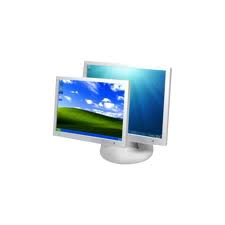
\includegraphics[width=.2\paperwidth]{images/vm.jpg}}
			\pause \centering{ {\Huge +} }
				\makebox[\textwidth]{
\includegraphics[width=.2\paperwidth]{images/cloud-server1.jpg}}
			\pause \centering{ {\Huge = ?}}
		\end{column}
		\begin{column}{.5\textwidth}
			\pause
			\begin{itemize}
				\item Policy enforcement?
				\item Storage agnosticity?
			\end{itemize}
		\end{column}
	\end{columns}

\end{frame}

\begin{frame}{Our solution}

	{\Large Archipelago}

	\makebox[\textwidth]{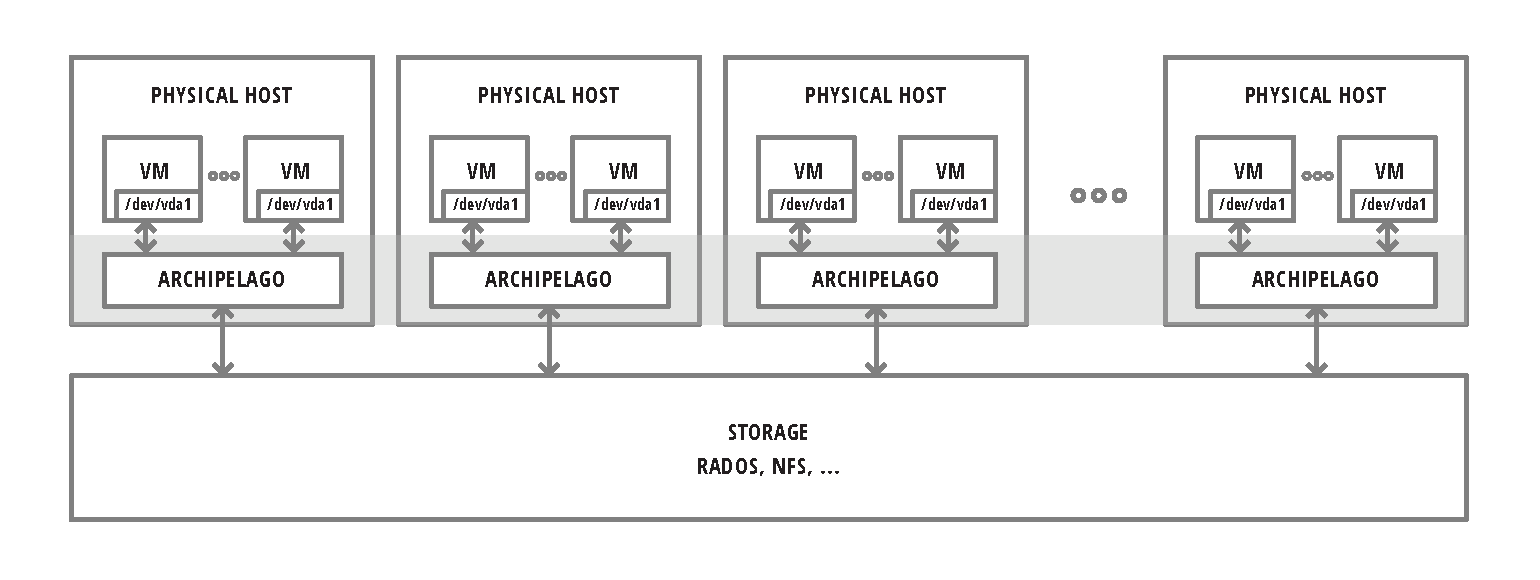
\includegraphics[width=\textwidth]{images/archipelago_overview_a.pdf}}

	\spc

	Key features:
		1) Software-defined
		2) Distributed
		) Modular
		Copy-On-Write
		Storage agnostic

	\note{Η λύση που χρησιμοποιήσαμε είναι το Archipelago}
	\note{
		\begin{itemize}
			\item Software-defined: αν και είναι ένα όρος 
				μαρκετινγκ, εμείς κανονικά. Σημαίνει με το 
				software ΟΡΙΖΕΙΣ το storage (εφαρμογή policy, 
				αλλαγή πορείας του request)
			\item τρέχει σε πολλούς κόμβους
			\item αποτελείται από διακριτά κομμάτια
			\item κάνει CoW (εξήγησε ότι τα images είναι λίγα, τα
				VMs πολλά, όπως όταν ένα process κάνει fork)
			\item μπορούμε χρησιμοποιήσουμε ότι θέλουμε
		\end{itemize}
	}

\end{frame}

\begin{frame}{Archipelago Architecture}
	%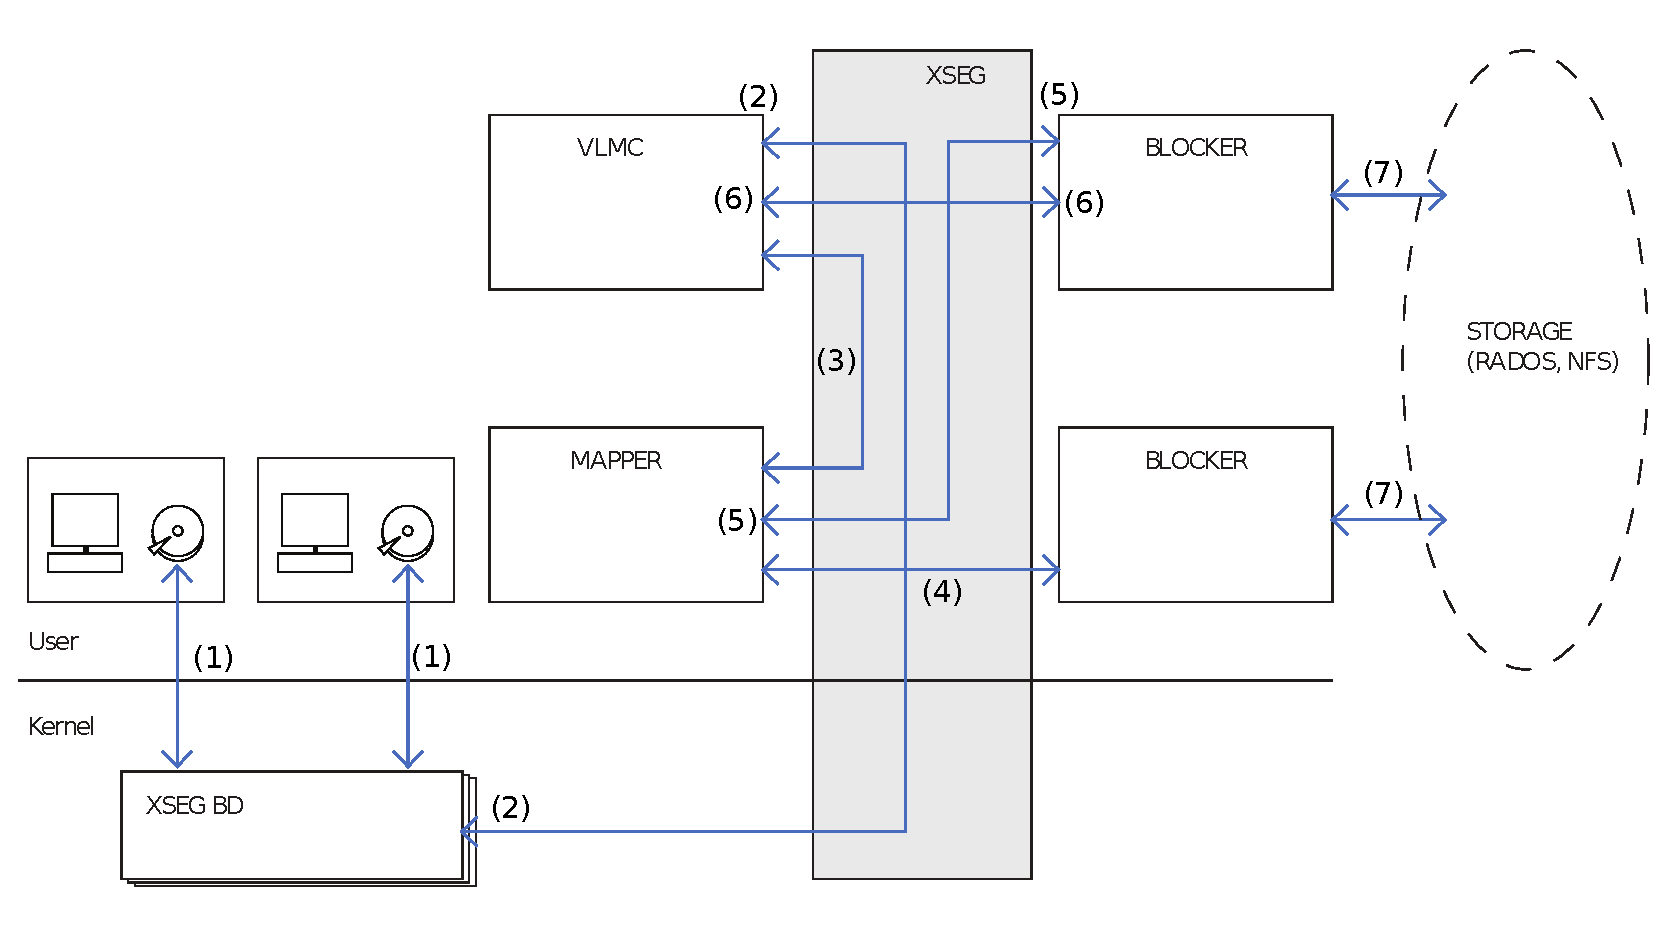
\includegraphics[{images/new_sxima_numbered.pdf}
	\begin{center}
		  \makebox[\textwidth]{\includegraphics[width=0.9\paperwidth]{images/new_sxima_numbered.pdf}}
	\end{center}

	\note[item]{To VM στέλνει αίτημα στο δίσκο του, ο δίσκος είναι εικονικός, 
		θα το δει ο hypervisor (εξήγησε τι είναι ο hypervisor) και θα το 
		στείλει στον δίσκο που το έχουμε πει. (xsegbd)}
	\note[item]{Ο xsegbd στέλνει τo αίτημα στο userspace κομμάτι του 
		Αρχιπελάγους το οποίο αποφαίνεται για τα αντικείμενα τα οποία 
		αντιστοιχούν στο αίτημα}
	\note[item]{μετά τα ζητάει από το storage μέσω των blockers}
\end{frame}

\begin{frame}{RADOS}

	The object store component of Ceph filesystem.\\
	\spc
	Key features:
	\begin{itemize}
		\item Replication
		\item Fault tolerance
		\item Self-management
		\item Scalability
	\end{itemize}


	\pause

	\spc
	Speed issues:\\
	VM with page-cache: > 90MB/s, < 1ms\\
	VM without page-cache: < 7MB/s, ~ 10ms

	\pause

	\spc
	Thesis goal: make this faster.

\end{frame}


\section{Caching}

\begin{frame}{Intro}

	Solution: Caching\\
	\spc
	Caching is:
	\begin{itemize}
		\item We have a slow medium
		\item Add a fast medium in a data path
		\item Transparently store the data that are intended for the 
			slower medium.
		\item Profit: later accesses to the same data are faster
	\end{itemize}
	\dspc
	Sounds familiar?
\end{frame}

\begin{frame}
	\makebox[\textwidth]{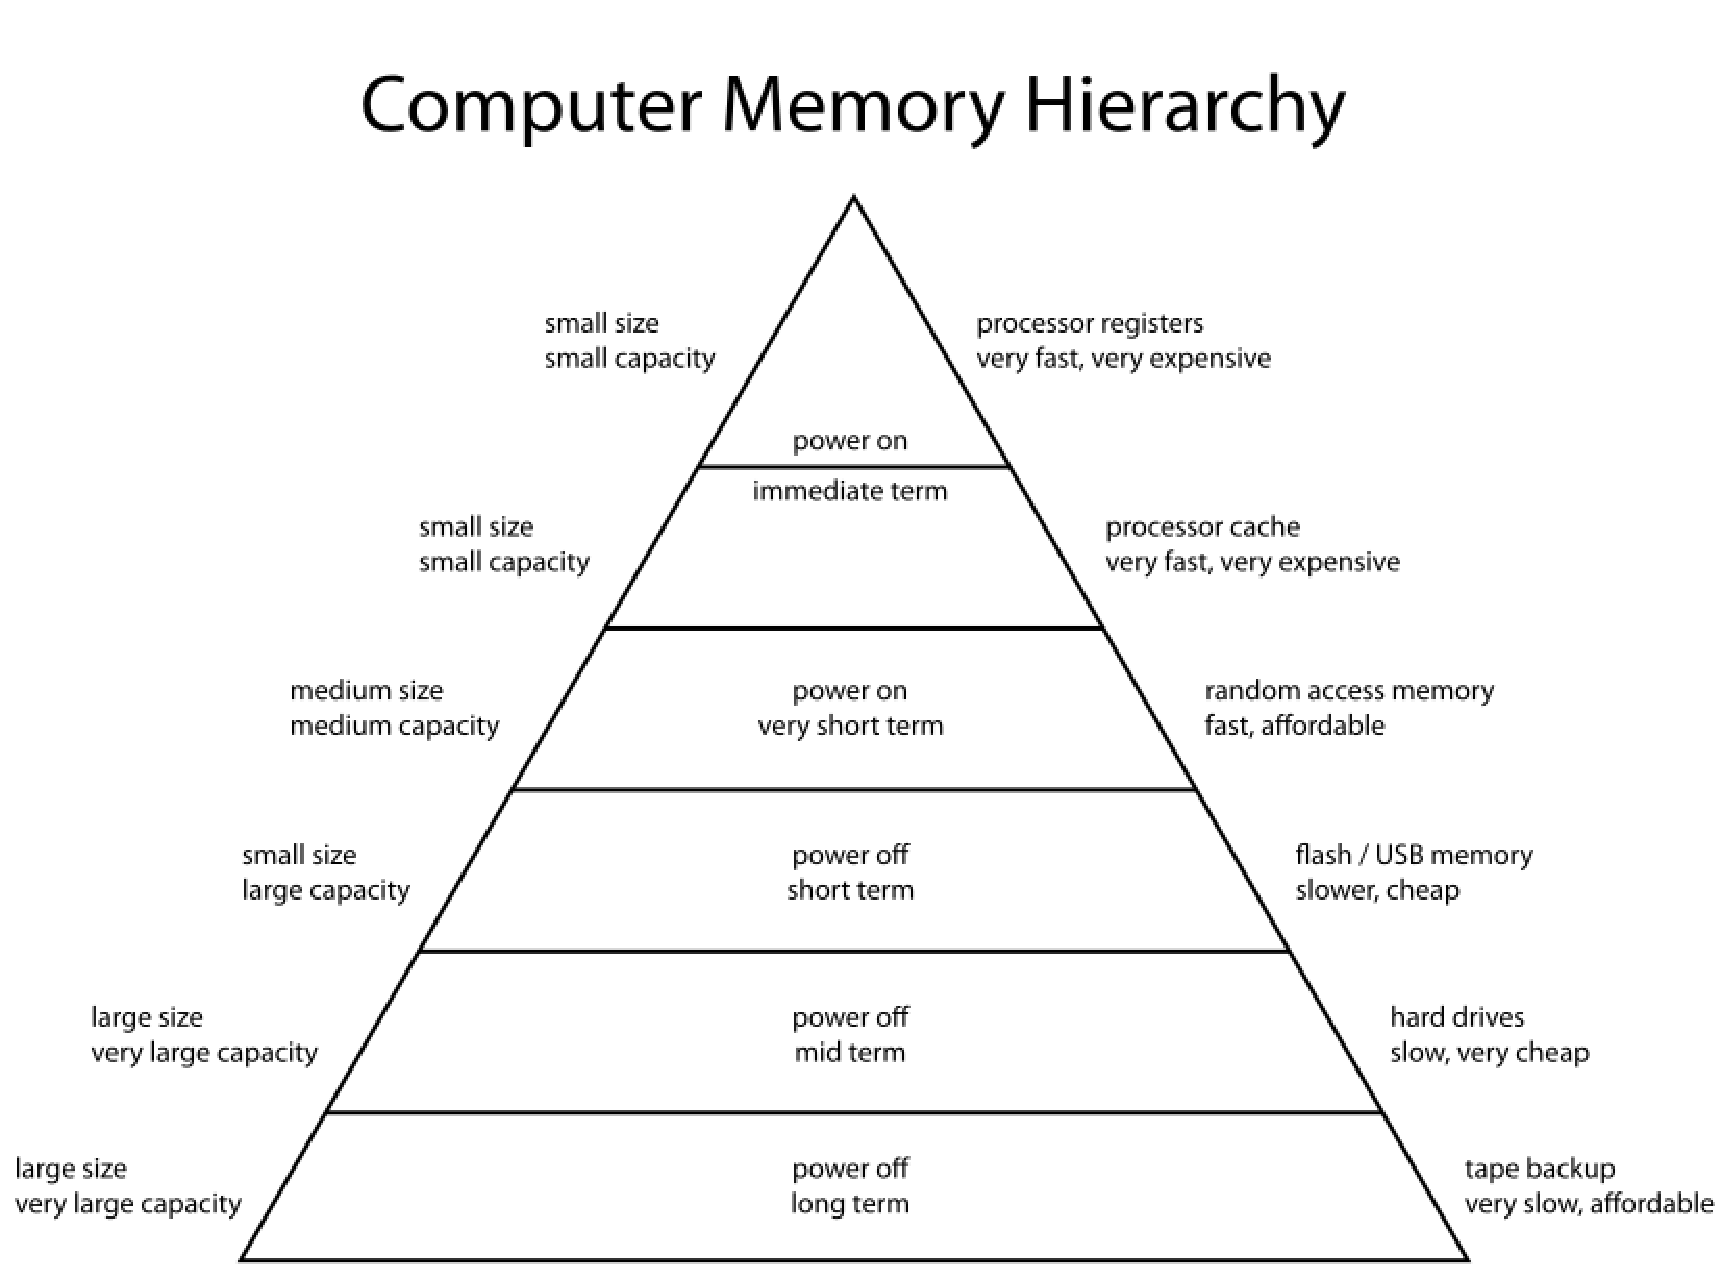
\includegraphics[width=0.8\textwidth]{images/mem-hier.pdf}}
	
	That's because every PC is built that way.
\end{frame}

\begin{frame}
	Is there anything to help us?
	\dspc
	We are not the first to have speed issues
	\dspc
	Facebook, Twitter, Dropbox, every one has hit and surpassed their 
	limits.
	\dspc
	There are solutions separated in two categories:
	\begin{itemize}
		\item Block store
		\item Key-value store
	\end{itemize}
\end{frame}

\begin{frame}{Block-store caching solutions}

	Most notable examples:
	\begin{itemize}
		\item Bcache
		\item Flashcache
		\item EnhanceIO
	\end{itemize}
	\dspc
	Typically scale-up solutions.
	\dspc
	Pros: Simple, scale-up\\
	Cons: Unaware of CoW, kernel solutions
\end{frame}

\begin{frame}{Key-value caching solutions}
	Most notable examples:
	\begin{itemize}
		\item Memcached
		\item Couchbase
	\end{itemize}
	\dspc
	Typically scale-out solutions
	\dspc
	Pros: Distributed with no SPOF, can utilize unneeded RAM\\
	Cons: Memcached has no persistence, Couchbase cannot use RADOS as its 
	backend, more suitable for databases
\end{frame}

\begin{frame}{Page-cache}

	What if we used the page-cache?

	\dspc
	Pros: Easy to activate, tested, very fast\\
	Cons: Unaware of CoW, no control over it, practically kernel solution\\

\end{frame}

\begin{frame}{Conclusions}

	\begin{itemize}
		\item Most solutions far from Archipelago's logic
		\item Block store might be good for the storage backend
		\item Must implement our own solution
	\end{itemize}
\end{frame}
	

\chapter{Design of cached}\label{ch:cached-design}

In the previous chapters, we have addressed the need for tiering in terms of
scalability as well as performance. % Which are these chapters? Link them.

We have also evaluated current caching solutions and described why they couldn't 
be used as a cache tier in Archipelago. % Provide link to a table of comparisons

With the results of chapter ? in mind, we can provide some more strict 
requirements that our solution must have:

% List the requirements for our solution
\begin{enumerate}
	\item \textbf{Nativity:} Our solution must be native to Archipelago i.e.  
		not need any translation layers to communicate with it.
		%explain why
	\item \textbf{Pluggability:} Our solution must be able to provide a 
		caching layer between peers that are already in operating mode 
		without restarting Archipelago. Also, it must be removed 
		without disturbing the service.
	\item \textbf{In-memory:} Our solution must cache requests in RAM, 
		since the next fastest tier, SSDs, are already being used in 
		RADOS as a journal.
\end{enumerate}

For the following chapters, we will drop the \textit{"solution"} moniker and we 
will use instead the proper name of our implementation, "cached", which simply 
means \textbf{cache d}aemon).

The following two chapters are the main bulk of this thesis and they present our 
own implementation that aims to fill the above requirements.

% Foretell what the following sections will contain
More specifically, this chapter provides an in-depth description of the design 
of cached. Section \ref{sec:rationale-design} provides the design rationale of 
cached and explains how its design meets the above requirements. Section 
\ref{sec:comp-design} presents the building blocks of cached while Sections 
\ref{sec:xcache-design}, \ref{sec:xworkq-design} and \ref{sec:xwaitq-design} 
provide a detailed explanation of their design. Section \ref{sec:cached-design}  
presents the interaction between cached and its  as well as the unique 
components that cached consists of.  Finally, in Section ?  we illustrate the 
flow of requests for cached.

\section{Design rationale}\label{sec:rationale-design}

One of the first architectural decisions was to implement cached as an 
Archipelago user-space peer (see Section \ref{sec:arch-peer} about Archipelago 
peers). This choice was the most natural one since it provides the smallest 
possible communication overhead with the other Archipelago peers. Also, this 
design decision covers the nativity requirement we posed at the beginning of 
this chapter.

The above design choice has another advantage too; we can register on-line the 
cached peer between the vlmc and blocker and unregister it when we want to.  
This opens up numerous possibilities such as plugging cached for 
QoS\footnote{Quality of Service} reasons when there is a peak in I/O requests.  
This is possible because, as we have mentioned in Section \ref{sec:arch-ipc}, 
XSEG ports can be registered on-line. Thus, during normal operation, the 
administrator can add the cached port to the request path between vlmc and 
blocker, and all requests will seamlessly be intercepted by cached. This 
follows the same principle with bcache, which plugs its own request\_fn() 
function to the virtual device it creates.  Unlike bcache however, cached can 
be plugged on and off at any time.

This also means that the pluggability requirement is also being met.

The next important design decision was what will cached index. Given that it 
will reside between the vlmc and blocker, where the VM's requests have already 
been translated to object requests, the natural choice is to cache objects.  

The decision to cache objects not only is the most natural one, but also is 
closer to the way our storage (RADOS) handles data. To understand the 
importance of it, consider the following:

Like bcache, our implementation must not only cache object requests fast but 
also try to coalesce them so that, when needed, they will be flushed to the 
slower medium in a more sequential fashion. The fact however that the VMs' 
volumes are partitioned into different objects, means that sequential data (in 
volume context) which reside in different objects will probably not be 
sequential in the storage backend too.

Thus, unlike bcache which expects that the backing device is also the physical 
device and coalesces date accordingly, our implementation is limited only in 
coalescing data in the object range (commonly 4MBs). If our implementation was 
caching in block or volume level, it would be unaware of that fact. 

Having decided that cached will cache objects, the next step is to decide
\begin{inparaenum}[i)]
\item on the index mechanism and
\item on what \textbf{exactly} would we index.
\end{inparaenum}

As for what we would index, it would be an overkill to further partition the 
objects and index regions within them. Moreover, this would make sense only if 
the objects where large (e.g. like volumes). So, our index mechanism should 
index object names solely. As for the index mechanism, we have chosen to use a 
very fast in-memory hash-table for this job. This covers the in-memory 
requirement we have set above. Also, this choice is one of the main reasons 
that our implementation is O(1).

Finally, another important decision was whether cached would be a 
multi-threaded peer. We have decided that we will implement it this way and 
then evaluate the performance of the implementation to find out if we are 
benefited by multi-threading or not.

Thus, cached must be able to work with multiple threads which will accept 
requests from cached's request queue and serve them concurrently with the other 
threads. Of course, multi-threading can be very tricky, especially when we are 
dealing with I/O requests and simultaneous accesses to the same object blocks.  
So, in order to achieve a balance between safety and speed, we use a
fine-grained locking scheme in critical sections that can be seen is discussed 
in detail in Section \ref{sec:xworkq-design}.

\section{Cached components}\label{sec:comp-design}

At this point, we must do an intermission before we show the design of cached.  
Specifically, we will show first the design of the cached's components, since 
many cached operations rely on them and the reader needs prior knowledge of 
them to grasp the cached design.

\subsection{Overview}

In this section, we will list the main components that cached relies on. Per 
Archipelago policy, most of these components have been written in the xtypes 
fashion (see Section \ref{arch-xtypes} about xtypes).  

The components of cached can be seen below:
 
% TODO: Link List to the definitions
\begin{itemize}
	\item xcache, an xtype that provides indexing support, amongst many 
		other things
	\item xworkq, an xtype that guarantees atomicity for execution of jobs 
		on the same object
	\item xwaitq, an xtype that allows conditional execution of jobs
\end{itemize}

and their design will be discussed in-depth in the following sections.

Also, we must note that the above components predate our cached implementation 
and are not a contribution of this thesis\footnote{xcache is an exception since 
	we have extended its functionalities for our purposes}. They are 
presented however in this thesis for clarity reasons. 

\subsection{The xcache xtype}\label{sec:xcache-design}

xcache is the most important component of cached. It is responsible for several 
key aspects of caching such as:

\begin{itemize}
	\item entry indexing,
	\item entry eviction,
	\item concurrency control and
	\item event hooks
\end{itemize}

Below, we can see a design graph of xcache:

\fixme add Figure here

% While explaining, point to the diagram objects, a, b, c etc.
\fixme add better design explanation \\
As we can see above, xcache utilizes two hash tables. One hash table is 
responsible for indexing entries (or more generally speaking "cache entries") 
that are active in cache.  The other hash table is responsible for indexing 
evicted cache entries that have pending jobs.  Again, more generally speaking, 
evicted cache entries are entries whose refcount has not dropped to zero yet.

On the following subsections, we present the features of xcache as well as 
their design.

\subsubsection{Entry Preallocation}\label{sec:xcache-entry-design}

Since xcache indexes a bounded number of entries, there is no need to allocate 
them on-the fly using malloc/free. Considering that we are caching at RAM level 
and not at SSD level, the system call overhead will have a considerable impact 
on performance. Thus, in our case, we pre-allocate the necessary space in 
advance and store them in a cache-node pool (note that this is different from 
the bucket pool).

\subsubsection{Entry indexing}\label{sec:xcache-index-design}

The index mechanism that xcache uses is a hash table named xhash, also an 
xtype. The reason why a hash table is used as an index mechanism is because:

\begin{enumerate}
	\item Given that we index only a certain number of entries, we expect 
		the that the insert, lookup and delete operations are in 
		constant time (see below for an explanation why)
	\item Hash tables can preallocate the space needed whereas 
		tries/b-trees/bst will allocate nodes as new entries are 
		inserted. Again, the fact that we index a certain number of 
		entries means that we expect that we will have many evictions 
		and insertions.
	\item We don't need to do substring matches (advantage of tries)
	\item We don't need to traverse the entries sequentially (advantage of 
		B-trees and BSTs)
\end{enumerate}

The hash table that is used is heavily based on dictobject\cite{dictobject},
the Python dictionary implementation in C. Distobject has been created to 
minimize the collisions and the hops (\fixme Explain that better). Its only 
drawback is that it needs to resize when the table's entry history has reached 
the 2/3 of its capacity.

Besides the hash table, which answers to the question "Where is the entry?" we 
also need another mechanism to answer the question "Is the entry still 
referenced?". xcache has such a mechanism which is commonly called "reference 
counting". Specifically, each entry has a counter that is 
incremented/decremented when a user accesses/releases an entry.

To sum up, when an entry is inserted, we use its name as a key and we update 
its refcount to 2, one reference from the user and one standard reference from 
the hash table. When we lookup for an entry, we use the entry's name as a key 
and then increment by 1 its refcount. 

\subsubsection{Entry eviction}\label{xcache-eviction-design}

The decision to have xcache index a bounded number of entries means that when 
it reaches its maximum capacity and is requested to index a new entry, it has 
to resort to the eviction of a previously cached entry. Evicted entries are not 
removed immediately from xcache. They are instead set in an "evicted" state and 
they reside in a special-purpose hash table until the user confirms that they 
can be removed. 

xcache handles evictions in an interesting way. More specifically, evictions 
occur implicitly and not explicitly, meaning that the user (peer) doesn't have 
to evict entries manually. For example, when a user tries to insert a new entry 
to an already full cache, the insertion will succeed and the user will not be 
prompted to evict an entry manually. Moreover, the user will be notified via 
specific event hook that is triggered upon eviction.

The scheme of implicit evictions and later on notification of the user has the 
advantage that lookups, inserts and evictions can occur atomically by xcache.  
This wouldn't be the case if the user was responsible for the evictions.

As for the eviction strategy, we have utilized an LRU queue. Not only it's 
optimal (\fixme verify it) for our purposes, but we have also mitigated the 
cost of keeping the last references for each entry by creating a simple LRU 
algorithm, which has O(1) complexity for all update actions. More about the 
implementation of the LRU algorithm can be found in Section 
\ref{xcache-evict-imp}.

\subsubsection{Concurrency control}

The concept of concurrency control has been discussed in chapter ?. The goal of 
xcache is to handle safely - and preferably fast - simultaneous accesses to the 
shared memory.

In order to do so, we must first identify which are the critical sections of 
xcache, to wit, the sections where a thread modifies a shared structure. These 
sections are the following:

\begin{itemize}
	\item
		\textbf{Most xhash operations:} Inserts and removals can modify 
		the hash table (e.g. they can resize it, add more entries or 
		delete existing ones). This also means that lookups must not 
		run simultaneously with the above two operations.
	\item
		\textbf{Cache node claiming:} Before an entry is inserted, it 
		must	acquire one of the pre-allocated nodes from the 
		cache-node pool and we must ensure that this can happen 
		concurrently from all threads.
	\item
		\textbf{Entry migration:} An entry can migrate from one hash 
		table to the other e.g. on cache eviction. This migration 
		involves a series of xhash operations; removal from one hash 
		table and subsequent insertion to the other. These two 
		operations must occur atomically.
	\item
		\textbf{Reference counting:} Every entry must have a reference 
		counter.  Reference counters provide a simple way to determine 
		when an entry can be safely removed. Since many threads can 
		have access to the same entry, we must provide a way to update 
		the reference counters atomically.
	\item
		\textbf{LRU updates:} Most actions that involve cache entries 
		must subsequently update the LRU queue. The updates at the LRU 
		queue must also occur atomically.
\end{itemize}

Let's see what guarantees we provide for each of the above scenarios:

\begin{itemize}
	\item
		\textbf{xhash operations:} We provide a lock for each hash 
		table. Only one thread can access each hash table at any time.
	\item
		\textbf{Cache node claiming:} The cache-node queue, is also 
		protected by a lock.
	\item
		\textbf{Entry migration:} When an entry is migrated from one 
		hash table to the other, we always acquire the lock of the hash 
		table of active entries and then the lock of the hash table of 
		the evicted entries. The order on which we take the locks is 
		very strict to avoid deadlocks.
	\item
		\textbf{Reference counting:} For the atomic increases and 
		decreases of a counter, we don't need a lock and its added 
		overhead. Instead, we can use the atomic get and atomic put 
		operations that the CPU provides.
	\item
		\textbf{LRU updates:} Since the majority of LRU updates take
		place when a new entry is inserted in the hash table, we can 
		protect our LRU under the same cache lock.
\end{itemize}

\subsubsection{Re-insertion}

We have previously mentioned that in xcache, there can be data migration 
between hash tables. Most commonly, an entry that is evicted from the active 
cache entries migrates to the hash table of the evicted cache entries, until 
its reference count falls to zero and can be freed.

However, what happens when xcache receives a request for an evicted entry which 
hasn't been freed yet? 

In this case, the entry switches state again and is inserted back to the hash 
table of active entries. Also, its reference counter is incremented accordingly 
in order not to be freed amidst this process.

This way, we can avoid waiting for an entry that has just been evicted to flush 
its data. 

\subsubsection{Event hooks}\label{sec:xcache-hooks-design}

Since xcache is created to provide core caching functionalities for other 
peers, it must also notify them when it takes an implicit action that the peer 
is not aware of. In Section \ref{xcache-eviction-design} we have seen one 
implicit action that xccahe takes when a user inserts an entry, namely 
eviction. 

Besides this event, there are others. The complete list is the following:

\begin{description}
\item[cache node initialization:]
	This hook is triggered when a cache node is initialized. It is 
	triggered once only for each node, during the initialization phase of 
	xcache.
\item[cache entry initialization:]
	This hook is triggered when a cache entry has been inserted in the 
	cache.
\item[cache entry eviction:]
	This hook is triggered when a cache entry has been evicted from the 
	cache.
\item[cache entry reinsertion:]
	This hook is triggered when an evicted entry has been reinserted in the 
	cache.
\item[cache entry finalization:]
	This hook is triggered when an evicted entry's refcount has dropped to 
	0. This serves as a warning for the user who has the opportunity to let 
	the cache entry go or increment its refcount.
\item[cache entry put:]
	This hook is triggered when an evicted entry has been totally removed 
	from the cache.
\item[cache entry free:]
	This hook is triggered when a removed entry's cache node has been sent 
	back to the cache node pool.
\end{description}

For each of the above events, we have created the respective event hook. The 
peer that uses xcache may choose, if it wants, to use them and if so, it can 
plug its own event function for each hook which will be called when the event 
is triggered.

\subsection{xcache flow}

To make the way xcache works a bit more clearer, we will see the flow for three 
of the main xcache operations; lookup of an entry; insertion of a new entry and 
removal of an entry:

\subsubsection{Insertion}

\fixme add figure and explanation

\subsubsection{Lookup}

\fixme add figure and explanation

\subsubsection{Put}

\fixme add figure and explanation

\subsection{The xworkq xtype}\label{sec:xworkq-design}

The xworkq xtype is a useful abstraction for concurrency control. Its purpose 
is to enqueue "jobs" (protected by a lock) and ensure that only one thread will 
execute them. There is no distinction as to which thread this will be, as well 
as no execution condition. The executive thread is simply the one that acquires 
the lock first.

xworkq is generally used when multiple threads want simultaneous access to a 
critical section. Instead of spinning indefinitely, waiting for a thread to 
finish, they can enqueue their job in the xworkq and resume processing other 
requests. xworkq is also generic by nature, since the "job" is simply a target 
function and its input data.

On the following figure, we can see the design of xworkq:

% Design of xworkq
\fixme add figure

It consists of a queue where jobs are enqueued.  The thread that enqueues a job 
can attempt to execute it too, by acquiring a lock for the xworkq. If the lock 
is unheld, the thread will acquire and will be able to execute the enqueued 
job. Else, it can safely leave and its job will be executed by the thread that 
has holds the lock.

In cached context, every object has an xworkq. Whenever a new request is 
accepted/received for an object, it is enqueued in the xworkq and we are thus 
ensured that only one thread at a time can have access to the object's data and 
metadata.

\subsection{The xwaitq xtype}\label{sec:xwaitq-design}

The xwaitq xtype bears some similarities to the xworkq xtype. Like xworkq, it 
is also an abstraction where "jobs" are enqueued and dequeued later on to be 
executed. Unlike xworkq though, jobs are executed only when a predefined 
condition is met. Another distinction is that the jobs in xwaitq are considered 
to be thread-safe and can be executed concurrently by any thread.  

xwaitq is commonly used in non-critical code sections that can be executed only 
under specific, predefined circumstances. The "jobs" that are enqueued in 
xwaitq are the same as the jobs of xworkq.

% Design of xwaitq
\fixme add figure

Unlike xworkq, before a job is enqueued, the thread can attempt to execute it 
by checking the execution condition. Only if the condition is \textbf{not} met 
does the thread enqueue the job to the queue. Before the thread leaves, it 
"signals" the queue and essentially rechecks the condition to ensure that it 
can't be executed. It can then safely leave since its job will be executed when 
another thread signals the queue successfully.

In cached context, xwaitqs are used to enqueue jobs which cannot be executed 
immediately. Common cases are when we have run out of space, when we have run 
out of requests etc.

\section{Cached Design}\label{sec:cached-design}

At this point, we have discussed in length the design of the cached components.  
Having the above sections in mind, we can proceed with presenting how cached 
has been designed.

Cached has been been designed mainly as the orchestrator, a peer that utilizes 
several different components to handle various tasks such as indexing (xcache), 
concurrency (xworkq) and deferred/conditional execution (xwaitq). Cached 
however is not limited to the above role as these components do not cover all 
of the needed tasks. There are several other key tasks that cached must 
undertake, namely:

\begin{enumerate}
	\item Request handling
	\item Write policy enforcing
	\item Cache coherence
\end{enumerate}

Moreover, cached extends its repertoire using some unique components, namely:

\begin{enumerate}
	\item Bucket pool
	\item Cache-IO
	\item Book-keeping
\end{enumerate}

We will illustrate the design of cached from two different perspectives: the 
operational perspective, which can be seen in Figure 
\ref{fig:cached-design.pdf}, and the component perspective, which can be seen 
if Figure ?. Moreover, we will further explain how cached manages the above new 
components and tasks in the following sections.

\diagram{cached-design.pdf}{Cached design}

\fixme add component diagram for cached (xcache, xworkq, objects, buckets etc.)

\subsection{Request handling}

Cached operates as a peer that receives requests from the vlmc. The majority of 
these requests will be read/write requests, but there are other types of 
requests too such as copy requests (sent when an object is copied-on-write) and 
info requests i.e. queries on what is the size of an object. Each of these 
requests must be handled independently, using special-purpose functions.

Furthermore, cached will also issue requests to the blocker mainly on two 
occasions: when it flushes a dirty object and when operating in write-through 
mode.

This means that, cached must be able to categorize requests and send them to 
the appropriate functions. Moreover, it must be able to create requests of its 
own, as well as handle cases such as running out of requests.

\subsection{Write policy enforcing}\label{sec:cached-wcp-design}

The user defines beforehand what will the write policy of cached be. There are 
two options: write-through and write-back. These policies aren't new and have 
already been discussed in chapter ?, but let's see what these policies 
translate to in cached context.

\begin{itemize}
	\item
		In \textbf{write-back} mode, cached caches writes, immediately 
		serves the request back and marks the data as dirty. When a read 
		arrives, it either serves the request with the dirty data 
		(read-hit) or forwards the request to the storage peer and 
		caches the answer (read-miss).

		This policy is used when we want to improve read and write speed 
		and can sacrifice data safety.
	\item
		In \textbf{write-through} mode, cached forwards writes to 
		blocker, servers the request when blocker replies, caches the 
		data and marks them as valid.  When a read arrives, it either 
		serves the request with the valid data (read-hit) or forwards 
		the request to the storage peer and caches the answer 
		(read-miss).

		This policy is used when we want to improve read speed and want 
		to make sure that no data will be lost.
\end{itemize}	

These policies are specified once during cached's deployment and cannot be 
switched on/off later on.

\subsection{Cache coherence}

Cache coherence is a concept that is closely connected with concurrency 
control, as is evident in Figure \ref{fig:cached-design.pdf}. It is commonly 
used as a term in the literature on the subject of caches for multiprocessor 
systems or distributed caches and it refers to:

\begin{enumerate}
	\item the consistency of data that are stored in the cache and
	\item how each change is propagated through the system, to the other 
		storage tiers.\label{list:second-coherence}
\end{enumerate}

If we wanted to rephrase the above to match our case, we could say that it 
refers to the consistency of the data that are stored in cached and how each 
change is propagated to the blocker.

The consistency of the cached data is greatly secured using the xworkq as the 
guard of parallel accesses to the object's data. However, the guarantee that 
data updates are conducted serially does not suffice for the consistency 
requirement.

The problem is evident if you consider the eviction of an object with dirty 
data. xcache does not operate on object level and thus is unaware of the 
contents of the cache entry. Thus, cached must use the cache entry finalization 
hook to increment the refcount of the object so that it can not be removed 
until all data have been flushed to the blocker. Essentially, cached overrides 
the xcache's book-keeping to maintain cache coherency.

The propagation of the data to the blocker is solely cached's job. One might 
consider that flushing the dirty data of an object would be sufficient to 
propagate the changes to the blocker. However, consider the scenario when an 
object is evicted and then subsequently reinserted, overwritten and evicted 
again. The result would be two flush requests, for the same data, sent to the 
blocker. Although the blocker guarantees that there will be no page-tearing, we 
cannot be sure about the order on which the data will be written.

To solve this problem, flush jobs must be deferred (using an xwaitq) if another 
flush for the same object is in flight. 

\subsection{Bucket pool}

% Explain what buckets are:
% a) That they are bounded
% b) That they have states
% c) That they are preallocated and every thread enqueues and dequeues an index 
% to them

We have already explained in Section \ref{sec:rationale-design} the reason why 
cached caches objects. There is, however, one important design issue that we 
must address. The issue is how will cached perceive the object's data. To make 
it a bit clearer, given that an object typically has 4MB of size, what should 
cached do when a user requests e.g. a 16KB chunk of it?

If we perceived the object's data as a monolithic chunk, we would need to read 
and cache the whole object just to reply to the user's request. If the user 
then requests a chunk from another object, we would have to cache that object 
too and in the end, we would thrash our cache
\footnote{
	cache thrashing occurs when we aggressively cache data that is only 
	used once and effectively leads to a snowball of evictions
}.

The solution we propose is to further divide objects to the next and final 
logical entity, \emph{buckets} (typically 4KB of size). Each bucket consists of 
its data and metadata and cannot be half-empty, or half-allocated. This way, we 
can also know which parts of the cached object are actually written, or are in 
the process of being read etc.

Thus, our solution to the hypothetical problem we have posed above is to 
request 16KB from the blocker, store the result in 4 buckets and then respond 
the request to the user.

The above answer, however, is not entirely complete. It implies that buckets 
are something readily available or attached to the object. Although each object 
\textit{could} have its buckets pre-allocated, this would limit the objects 
that we can cache since that, even if the user requested only a small chunk, 
each object would statically need 4MB of space.

Ideally, we would like to be able to cache thousands of objects but
\begin{inparaenum}[i)]
\item allocate a much smaller amount of buckets and
\item strictly when the user requests to.
\end{inparaenum}
To make things even faster, we would also like the buckets to be preallocated 
(like cache nodes in Section \ref{sec:xcache-entry-design}) to avoid the 
overhead of malloc/free system calls.

We have achieved the above by creating a bucket pool. The design of the bucket 
pool is the following:

\fixme add diagram

The bucket pool size is static and has been set during initialization by the 
administrator. After the necessary space has been allocated, it is divided in 
buckets and all the bucket indexes are pushed in a lock-protected stack (xq).  
Then, each thread can pop bucket indexes from the pool and attach them
to an object when needed. When that object is evicted, its attached buckets 
indexes are pushed back to the pool.

\subsection{Cache-IO}

When a request is accepted, all Archipelago peers commonly embed it in a peer 
request (you can see more about peer requests here ?). The peer request always 
holds the original request and optionally, several other fields that are of 
importance to the peer.

In our case, we keep in cached's peer requests a new structure called Cache-IO, 
on which we store the xcache handler of the request handler as well as the 
state of the request. Moreover, since the request may break internally in many 
others, we keep track of how many pending requests remain until the original 
one can be completed.

\subsection{Book-keeping}

In order to know when an object is in flushing state, when a bucket has been 
allocated or when a bucket is being read, cached must employ some sort of 
book-keeping of their states. The entities that require to track their states 
are:

\begin{enumerate}
\item \textbf{buckets:} Each bucket has two different states that must be 
	tracked. The first is its allocation state:
	\begin{enumerate}[i)]
		\item free, meaning that the bucket is not allocated
		\item claimed, meaning that the bucket is allocated
	\end{enumerate}
	The second is its data state:
	\begin{enumerate}[i)]
		\item invalid, meaning that it currently holds no data
		\item valid, meaning that it has data that correspond with the 
			blockers data
		\item loading, meaning that a read request has been sent to the 
			blocker to be filled with data
		\item dirty, meaning that it currently holds newer data that 
			what the blocker has.
	\end{enumerate}
\item \textbf{Objects:} The bucket states of an object provide a good 
	indication of the object's status, yet not a complete one. The statuses 
	we keep for the objects are:
	\begin{enumerate}[i)]
		\item ready, meaning that it is ready to accept data
		\item invalidated, meaning that it is not ready to accept data
		\item flushing, meaning that it is currently flushing dirty 
			data to the blocker
		\item failed, meaning that a request has failed for this object 
			and we must stop using it
	\end{enumerate}
\item \textbf{Cache-ios:} Cache-ios also have states. They are the 
	following:
	\begin{enumerate}[i)]
		\item accpted, meaning that the request has just been accepted
		\item reading, meaning that the request wants to read data
		\item writing, meaning that the request wants to write data
		\item served, meaning that the request has been served the data 
			it needed
		\item failed, meaning that the request has failed
	\end{enumerate}
\end{enumerate}

Moreover, we keep global and per-object counters of every object's bucket 
states. The benefits from this approach is that we can know at any time if an 
object (or cached in general) has a bucket in a certain state.

\section{Cached Operation}\label{sec:op-design}

\subsection{Write}

This is the flow for the write path:

\fixme add diagram and explanation

\subsection{Read}

This is the flow for the read path:

\fixme add diagram and explanation

\subsection{Copy}

This is the flow for the read path:

\fixme add diagram and explanation

\subsection{Info}

This is the flow for the read path:

\fixme add diagram and explanation


\chapter{Performance evaluation of cached}\label{ch:cached-evaluation}

\begin{flushright}
	\textit{"There are three kinds of lies:\\
		lies, damned lies, \\
		and \sout{statistics} benchmarks."}	\\

	Mark Twain (modernized)
\end{flushright}

It may seem as an ironic statement, considering that we are about to provide 
benchmark results for cached, but it's actually is a valid one.
\begin{comment}
What Mr.  Twain tries to say here
\footnote{
	and that's a phrase usually not heard in programming contexts...
}
is that the presentation of partials facts for something can be used to 
fabricate a plausible truth for it.
%This is shit, fix it
In science's case, it so often happens that promising results for an experiment 
can seem more important to the researcher's eye than negative ones due to 
positive reinforcement.
\end{comment}
In our case, we will try not to merely smear the next pages with diagrams but 
first explain the benchmarking methodology behind them and then provide a 
concrete depiction of cached's performance under various workloads.

The skeleton of this chapter is the following: Section \ref{sec:perf-meth} 
explains the methodology behind our measurements. Section \ref{sec:test-bed} 
provides details about the hardware on which we have conducted our benchmarks.  
Section \ref{sec:perf-plot} presents the results of the benchmarks that we have 
conducted and provides in-depth explanations about each of them.  Finally, 
Section ?  is reserved for cached on a VM (\fixme take these measurements).

\section{Benchmark methodology}\label{sec:perf-meth}

The benchmarks that have been executed and whose results are presented in this 
chapter, will be split in two categories, both of which have their own distinct 
goals:

The first category is the comparison between using cached \textbf{on top} of 
the sosd peer (sosd has been discussed here ? \fixme add section) and using 
solely the sosd peer.

\begin{comment}
The category's goal is to "defend" one of the core thesis arguments, that 
tiering is a key element that will improve the performance of Archipelago.  
\end{comment}

In order to effectively compare the performance of cached and sosd, we must 
consider the following: 

\begin{enumerate}
	\item The comparison of the two peers should try to focus on what is 
		the best performance that these peers can achieve for a series 
		of tough workloads.
	\item The circumstances under which both peers will be tested need not 
		be thorough but challenging. For example, it may be interesting 
		to test both peers against sequential requests, but
		\begin{inparaenum}[i)]
		\item such patterns are rarely a nuisance for production 
			environments
		\item they do not stress the peers enough to provide something 
			conclusive
		\item they are out of the scope of this section as there can be 
			many of these kinds of tests and adding them all here 
			will impede the document's readability.
		\end{inparaenum}
	\item Both peers must be tested under the same, reasonable workload, i.e a 
		workload that can be encountered in production environments.
	\item If the peer doesn't show a consistent behavior for a workload, it 
		must be depicted in the results.
\end{enumerate}

Having the above in mind, the next step is to choose a suitable workload.  This 
choice though is fairly straight-forward; in production environments, the most 
troublesome workload is the burst of small random reads/writes and is usually 
the most common one that is benchmarked.  

One may ponder however, how many requests can be considered as a "burst" or 
which block size is considered as "small". Of course, there is not only one 
answer to this question so, we will work with ranges. For our workload, we will 
use block sizes ranging from 4KB to 64KB and parallel requests ranging from 4 
to 16.

The second category deals solely with the inner-workings of cached and its 
behavior on different operation modes or states. Its aim is not to capture the 
performance against a tough workload, but to explain \textbf{why} this 
performance is observed and how each of the options affect it. In this 
category, we measure how threads impact the performance of cached or what 
impact (if any) does our index mechanism have.

Finally, in the following sections, for brevity reasons, we will talk about 
comparing cached and sosd. What the reader must keep in mind however is that 
cached is essentially the cache layer above sosd, which means that we actually 
test sosd vs cached over sosd.

\section{Specifications of test-bed}\label{sec:test-bed}

The specifications of the server on which we conducted our benchmarks is the 
following.

\begin{table}[H]
	\centering
	\begin{tabular}{ | l | l | }
		\hline
		Component & Description \\ \hline \hline
		CPU &  2 x Intel(R) Xeon(R) CPU E5645 @ 2.40GHz \cite{e5645} \\
		 & Each CPU has six cores with Hyper-Threading enabled, which equals to 
		 24 threads. \\ \hline
		RAΜ & 2 banks x 6 DIMMs PC3-10600 \\
		& Peak transfer rate: 10660 MB/s \\ \hline
	\end{tabular}
	\caption{Test-bed hardware specs}
	\label{tab:hardware-specs}
\end{table}

\begin{table}[H]
	\centering
	\begin{tabular}{ | l | l | }
		\hline
		Software & Version \\ \hline \hline
		OS &  Debian Squeeze \\ \hline
		Linux kernel & 3.2.0-0 (backported) \\ \hline
		GCC & Debian 4.4.5-8 \\ \hline
	\end{tabular}
	\caption{Test-bed software specs}
	\label{tab:software-specs}
\end{table}

\todo add configuration of RADOS cluster (journal, backing storage, network 
connection)

\fixme Mention that the peers were evaluated by sending requests directly at 
their ports.

\section{Performance comparison between cached and sosd}
\label{sec:perf-plot}

As mentioned above, for our first test, we will evaluate the read and write 
performance of cached and sosd for a random workload with parallel requests of 
small size. In order to measure accurately their performance, we will use two 
different metrics:

\begin{description}
	\item[Bandwidth:] \hfill \\
		Bandwidth measures the maximum throughput that the application 
		can sustain. This metric is usually used to indicate how much 
		I/O (from various inputs) can an application handle within a 
		second.
	\item[Latency:] \hfill \\
		Latency is the converse of bandwidth. It is a measurement from 
		the viewpoint of the issuer of requests and indicates the 
		responsiveness of the tested application. It is commonly 
		calculated as the average reply time for a series of requests.
\end{description}

On the following sections, we present the benchmarks that we conducted for the 
first category. The first benchmark, which is shown in Section 
\ref{sec:peak-plot} attempts to depict the behavior of cached during a peak of 
I/O requests. The second benchmark, which is shown in Section 
\ref{sec:sustained-plot}, illustrates the behavior of cached under continuous 
load.  On these sections, cached is always multi-threaded and uses 4 threads.

\subsection{Workload smaller than cache size - Peak behavior}
\label{sec:peak-plot}

We begin with the bandwidth performance of our peers. The write performance can 
be seen in Figure \ref{fig:bw-write-comp-lie.pdf} while the read performance 
can be seen in Figure \ref{fig:bw-read-comp-lie.pdf}.

Before we proceed with the interpretation of the diagram results, we will 
briefly comment on the diagram structure. Due to the fact that the performance 
of the two peers differs in at least two orders of magnitude, the results would 
look too flat in a conventional diagram that would scale from 0 to 11000. To 
amend this, we have broken the y-axis of our diagrams in two parts with 
different scales and starting values, in order to make the comparison easier to 
the eye.

\diagram{Comparison of bandwidth performance for write 
	peaks}{bw-write-comp-lie.pdf}
\diagram{Comparison of bandwidth performance for read 
	peaks}{bw-read-comp-lie.pdf}

The initial results look very promising. For write requests, the speedup for 
very small block sizes (4KB - 16KB) is approximately \textbf{100x} whereas for 
larger ones (32KB - 64KB) it ranges from \textbf{50x to 200x}. For read 
requests, the speedup for very small block sizes is approximately \textbf{50x}, 
whereas for larger block sizes, it ranges between \textbf{20x - 75x}.

These results not only illustrate the performance gap between RAM and
HDDs but also show that our implementation manages to keep its bandwidth 
consistently over 1 GB/s in stress scenarios. However, we must keep in mind 
that they only show a part of the full picture, since it does not show how 
cached behaves past its cache size.

Moreover, upon closer inspection the following questions arise:

\textbf{1) Where is the speedup difference between reads and writes attributed 
	to?}

We have mentioned above that the speedup for writes is between 50x and 200x 
whereas for reads is between 20x and 75x. Although it is a large speedup in 
both cases, it also shows some of the shortcomings of our implementation.

We attribute the speedup difference to three factors:

\begin{enumerate}
	\item The performance of cached is almost the same for writes and 
		reads.  This is expected behavior as the read and write paths 
		for cached have many common parts (\fixme show write/read path)
		\footnote{To be more strict, reading seems a bit faster than 
			writing, but that is probably attributed to CPU caches 
			and the fact that reading from RAM is a non-destructive 
			operation in contrast to writing.}.
	\item Cached doesn't scale much past the 16KB block size. This is an 
		interesting observation with an unexpected answer. It may seem 
		implausible at first, but what happens is that we are actually 
		hitting the bandwidth limit of the RAM modules. If we consult 
		the table \ref{tab:hardware-specs}, we can see that the 
		bandwidth limit of the RAM is about \mytilde10.7GB/s
		\footnote{A more careful look shows that we surpass this limit, 
			which is expected given the fact that we have a multi 
			channel RAM setup.}.
		This limit is approached asymptotically as the block size 
		increases and the index overhead decreases (more about the 
		index overhead later in the measurements of Section ? \fixme 
		add section).
	\item On reads, sosd is benefited from the existence of caches in 
		various levels e.g. on OSD level, on RAID controller level.
\end{enumerate}

To sum up, the cached's performance remains relatively the same in both reads 
and writes, it is merely the sosd that is getting faster in reads due to 
caches. 

\textbf{2) Why is cached's performance increased along with block size?}

We expected that sosd's performance would increase proportionally to the block 
size, due to the rotational nature of hard disk drives, but why does this 
affects cached too? It is certainly not attributed to any \texttt{memcpy()} 
performance tricks, since we always write in bucket granularity, which means 
that a 16KB write is translated to 4 x 4KB writes.

From this observation, we extrapolate that the CPU operations such as indexing,
job enqueuing, accepting and responding requests, that occur proportionally 
more times for smaller block sizes, dominate the cached's performance.

We can see this more clearly if we consult Table \ref{tab:2threads}.

\begin{table}[H]
	\centering
	\begin{tabular}{ | l | l | l | l | l |}
		\hline
		Bandwidth (MB/s) & IOPS	  & Latency (usec) & Iodepth& Block size (KB) \\ \hline \hline
  2652.327   &	678995.620& 5.002&	4&		4 \\ \hline
  4427.89l   &	566769.888& 6.176&	4&		8 \\ \hline
  5900.719   &	377646.042& 9.672&	4&		16 \\ \hline
  6895.167   &	220645.338& 17.179&	4&		32 \\ \hline
  7090.661   &	113450.584& 34.237&	4&		64 \\ \hline

	\end{tabular}
	\caption{Write performance results for 2-threaded cached}
	\label{tab:2threads}
\end{table}

\fixme elaborate on that

Merely using two threads instead of four lessens the performance gap 
significantly.

\textbf{3) Why cached's perforance does not improve proportionally to the 
	parallel requests?}

The reason why we see only a minor increase in the performance of cached, even 
though it is multi-threaded, is because our locking scheme is not fine-grained 
enough. We have a single lock for our request queue, a single lock for most of 
the hash table accesses and this inevitably causes a lot of threads to spin.  
This slight improvement we see is mainly due to the fact that requests are 
effectively being pipelined while waiting each other to release its lock.  

We now proceed to the latency results. The write performance can be seen in 
Figure \ref{fig:lat-write-comp-lie.pdf} while the read performance can be seen 
in Figure \ref{fig:lat-read-comp-lie.pdf}.

\diagram{Comparison of latency performance for write 
	peaks}{lat-write-comp-lie.pdf}
\diagram{Comparison of latency performance for read 
	peaks}{lat-read-comp-lie.pdf}

The latency results corroborate the observations that we made for the bandwidth 
results. As we can see, the latency of cached is proportional to the number of 
parallel requests, which reinforces the assumption that our locking scheme is 
not granular enough, whereas sosd has only a small variance.

\subsection{Workload larger than cache size - Sustained behavior}
\label{sec:sustained-plot}

We now proceed to the second part of the comparison between cached and sosd.  
On this part, we will once again evaluate their performance against a random 
workload with many parallel requests. Unlike the first part though, where the 
cache size was larger than the workload, on this part the cache size will
only be half of it. Having a smaller cache than the workload is after all the 
most common scenario for production environments and the results should 
complete the picture of cached's behavior in a production environment.

For this test, there are two main parameters we must take into account: the 
cache size and the maximum objects. These parameters have been decoupled in our 
implementation and we expect different results for each combination. More 
specifically, we have tested cached with half the workload size and:

\begin{enumerate}
	\item half the objects of the workload (referenced as 
		\textbf{cached-limited} from now on).
	\item more than the objects of the workload (referenced as 
		\textbf{cached-unlimited} from now on).
\end{enumerate}

Also, we have tested cached in write-through mode, to see its behavior in 
sustained writes. \fixme say it has unlimited objects 

Furthermore, for this benchmark, we tested only the write performance of cached 
and sosd.  Also, we chose to use 16 parallel requests and 4KB block sizes, 
since these seemed the most troublesome in the previous benchmark.

Before we proceed to the results, we must explain first how the diagrams below 
are structured. Since cached's performance is fairly unstable in this scenario, 
we have chosen to illustrate it as the benchmark progresses.  Thus, the x-axis 
shows what percent of the benchmark has been completed and for every 5\%, we 
show the performance of cached for that part.

The bandwidth results can be seen in Figure \ref{fig:bw-write-comp-truth.pdf}, 
while the latency results can be seen in Figure 
\ref{fig:lat-write-comp-truth.pdf}.  Due to the vast bandwidth drop of cached, 
the y-axis uses a logarithmic scale to show a more clear picture of what 
happens when the performance reaches the 10 MB/s mark.

\diagram{Comparison of bandwidth performance for sustained writes} 
{bw-write-comp-truth.pdf}

\diagram{Comparison of latency performance for sustained writes}
{lat-write-comp-truth.pdf}

This diagram has several interesting points which we will address below.

\textbf{1) Why cached-unlimited's performance drops in the middle of the 
	benchmark?}

Since cached-unlimited can index more objects than the workload, there is no 
need to evict entries from the hash table to insert new ones. Cached-limited on 
the other hand, has at any point a 50\% chance to receive a request for a 
target that does not index. Thus, when cached-unlimited starts to receive the 
first 50\% of requests, it only needs to store them and, as we have seen in the 
first part of this section, it does so very fast.

However, at around 50\% of the benchmark its space is depleted and thus, it has 
to manually evict entries. At this point, we see that its performance 
degenerates to the performance of cached-limited.

\textbf{2) Why cached-limited's performance is significantly less than the 
	sosd's performance?}

As we have explained above, cached-limited constantly evicts entries due to its 
object limitation. It may seem that the only cost of eviction is that the 
performance degenerates to the performance of sosd, but that is not entirely 
true.

When an entry is evicted, all of its contents must be flushed before the new 
entry can overwrite them. Moreover, the cost of concurrency control for hash 
table migrations and the cost of creating new requests and copying the data in 
them is not negligible. Finally, due to constant evictions, there are only a 
few buckets cached for any entry, which in turn does not leave any margin for 
coalescences.

\textbf{3) Why cached-unlimited's performance increases after the 50\% mark ?}

After the 50\% mark, cached-unlimited will have to resort to evictions in order 
to store new data. Unlike cached-limited though, cached-unlimited has already 
cached half of the workload's data, which allows for many coalescences.  
Moreover, cached evicts whole objects to get their buckets, which means that 
evictions will be less frequent that cached-limited, which evicts entries to 
index other entries.

\textbf{4) Why cached in write-through mode performs the same as sods?}

The performance of cached in write-through mode is the same as sosd's since 
write requests are essentially forwarded to sosd and are cached when sosd 
responds. The caching has no significant overhead, compared to the waiting time 
for sosd, since there are no dirty entries and thus no costly evictions.

What is more interesting however is the comparison of read performance between 
cached and sosd, which can be seen in Table \ref{tab:writethrough}.

\begin{table}[H]
	\centering
	\begin{tabular}{ | l | l | l | l | l | l |}
		\hline
		Peer& Bandwidth (MB/s) & IOPS	& Latency (usec) & Iodepth & Block size 
		(KB) \\
		\hline \hline
		sosd& 34.124&		8735.699&		1828.758&	16&		4 \\ \hline

		cached& 44.897&		11493.511&		1389.511&	16&		4 \\ \hline

	\end{tabular}
	\caption{Read performance comparison of cached in write-through mode and 
		sosd}
	\label{tab:writethrough}
\end{table}

The read performance of cached has a noticeable increase of 25\%. This is 
expected, since cached serves read requests either from its cached data or from 
sosd. This means that it has the baseline performance of sosd plus the extra 
performance gain from cache hits.

\section{Performance evaluation of cached internals}

To some extent, we have already discussed about the behavior of cached when we 
tweak various of its parameters, such as the over-subscription of its objects, 
the cache size or its write policy. In this category, we will further solidify 
our previous assumptions about the inner workings of cached by measuring:

\begin{enumerate}
	\item how cached scales with the number of threads
	\item the overhead of the index mechanism
\end{enumerate}

Note that the tests will be run with the following parameters:

\begin{description}
	\item[Mode] Write-back
	\item[Block size] 4KB
	\item[Cache size] Always larger than benchmark size
	\item[Operation] Writes
\end{description}

The above options have been chosen to isolate cached of any other factors that 
may alter its performance, such as evictions and delays due to sosd.

\subsection{Cached performance per number of threads}

Measuring the performance impact of multi-threading is nonsensical, if the 
application is not tested against many parallel requests. Hence, we will test 
each n-threaded cached configuration against a range of parallel requests and 
measure its performance.

The bandwidth results can be seen in Figure \ref{fig:bw-write-threads.pdf} 
whereas the latency results can be seen in Figure 
\ref{fig:lat-write-threads.pdf}.

\diagram{Bandwidth performance for each number of 
	threads}{bw-write-threads.pdf}
\diagram{Latency performance for each number of threads}{lat-write-threads.pdf}

From these results, we derive the following conclusions:

\begin{enumerate}
	\item Cached is generally benefited from multi-threading, when the amount 
		of parallel requests is more than two. More specifically, we achieve a 
		major performance improvement of up to 75\% when using two threads, as 
		well as a lower, but significant, performance improvement for up to 
		four threads, as the number of parallel requests increases.
	\item Cached does not scale well past four parallel requests, regardless of 
		the number of threads.
	\item Adding more than two threads degrades significantly the performance 
		of cached, when the number of parallel requests is small.
\end{enumerate}

Finally, these results, along with the results of the first part, clearly show 
that we cannot fully utilize the multi-threading capabilities of cached unless 
we employ a more fine-grained locking scheme.

\subsection{Cold cache vs Hot cache}

This scenario will attempt to evaluate the overhead of cache misses for 
\textbf{write} operations. Theoretically, this should account to the overhead 
of adding new entries to cached and consecutively, an indication of the 
complexity of our index mechanism.

Our experimental procedure is the following:

\begin{enumerate}
	\item We inserted 128K
		\footnote{where \textbf{K} is \textbf{x1024} objects}, 256K, 512K and 
		1M
		\footnote{where \textbf{M} is \textbf{x1024\textsuperscript{2}} 
			objects}
		objects in a cached peer configured to hold up to 2M objects and 
		measured their average latency times.
	\item Subsequently, we attempted to insert these objects in cached again 
		and measured their average latency times.
\end{enumerate}

The difference between the first and the second iteration is that in the second 
iteration, the objects are hot in the cache and thus cached will not need to 
reinsert them. This means that the first iteration has the extra actions of 
allocating the entries and inserting them in the cache, whereas the second 
iteration will only lookup the objects in the cache.

We expect that the extra indexing action will add a constant overhead to the 
measurements of the first iteration, regardless of the number of entries.
Moreover, the latency times for the second iteration should remain the same, 
regardless of the number of entries.

\textbf{Note:} To get the most accurate results and since we want to test just 
the overhead of our indexing mechanism, cached has been configured to use one 
thread.  Moreover, the I/O depth is also one, to make sure that latency times 
are not skewed by the time the request waits in the request queue.

We present the results on Figure \ref{fig:cold1.pdf}.

\diagram{Latency performance of cold/warm cache for various objects}{cold1.pdf}

The focal point in these results is that the write latency, either of cold or 
warm caches, remains practically the same as the number of objects increases.  
This reinforces our statement that cached has average case O(1) complexity.

Finally, an interesting finding from our results is that the latency of 
indexing an entry, even in a hash table that supports 2 million objects (and 
potentially 8TBs of data), is less than 1μs, which is a very strong feature of 
our implementation.

\begin{comment}
As a side note, we observe a constant decrease in writelatency as the number of 
objects increase this is not something that should be attributed to our 
implementation. (explain that we have used a hash table that holds 2million 
objects, so it is not mapped to our process's address space. When more objects 
are indexed, the hash table becomes fuller and the latency of mmap()s is 
equally distributed to the objects. Else, the hash table is more scarce but the 
same blocks are hit, albeit not fully written, and thus the mmap latency is the 
same but distributed to less objects.)
\end{comment}

\chapter{The Synapsed peer}

On the previous sections, we have evaluated the design of cached and we have 
seen that is heavily bounded by CPU. The implications of this, however,
are bigger, if we consider that all the Archipelago is running in the host 
machine, whose CPU's are already oversubscribed. This means that cached must 
compete for CPU time against the running VMs, essentialy defeating the QoS 
purpose it serves.

On the other hand, on the RADOS nodes, the CPUs are not used to the full 
potential. Thus, it would be interesting to check how well cached (and 
Archipelago in general) would behave, if the VM's data where send initially 
over network and then handled by the vlmc. So what we mean is to turn the 
current situation from how it is in Figure ? to the following:

\fixme add figure for network

To this end, we have created a network peer called synapsed (from 
\textbf{synapse d}aemon) as a proof-of-concept, that should be able to receive 
any type of requests and send them through the network to another Archipelago 
segment. We must note that this peer has not been created with performance in 
mind but its main aim is to provide the functionality needed for our purposes.  
As a consequence, we haven't used tools such as ZeroMQ or libevent that would 
boost the performance of the implementation.

More specifically, on Section...

\section{Design of synapsed}

Given that currently Archipelago is not network-aware, peers from one segment 
cannot know the ports of peers of another segment. Moreover, they cannot send a 
request to the synapsed peer and simultaneously target a peer in another 
segment. So, we are faced with the problem of what will be the limitations of 
synapsed.

We propose the following solution to this problem: Each of those two segments 
must have at least one synapsed peer. So, when one synapsed accepts an XSEG 
request, it will translate it to a network request, send it to the synapsed 
peer of the other segment which will finally translate it back to an XSEG 
request.  Moreover, each synapsed peer must be attached to a peer of its 
segment, which will serve as the request target when synapsed accepts request.  

This means that synapsed does not actually connect two remote segments
but bridge two remote peers over network.

The way synapsed handles requests can be seen in Figure ?

\fixme add figure

The main difficulty is to make synapsed listen from its port and its request 
queue simultaneously. We have tackled this problem in Section ?

Moreover, synapsed sends requests using bare TCP sockers, without using. This 
means that it handles the marshaling of requests, send/recv errors as well as 
polling by itself.

Finally, synapsed has been created as a single-threaded peer.

\section{Implementation of synapsed}

In the following sectionσ we will

\section{Synapsed initialization}

Synapsed is a much simpler peer than cached and requires only the following 
arguments.

\begin{description}
	\item[-hp] The port where it will listen for requests.
	\item[-ra] The remote address of the segment. \textbf{NOTE:} it can 
		point to the same segment, which means that synapsed provides a 
		generic way to bridge two peers who reside in the same host but 
		in a different segment.
	\item[-rp] The remote port of the other synapsed.
	\item[-txp] The XSEG port of the peer which synapsed will attach on
\end{description}

Having the above arguments, synapsed can create a socket and bing its port it.  

\section{Request polling}

Synapsed typically uses the common peer loop and Archipelago IPC methods to 
check its XSEG ports for new requests. However, it simultaneously needs to 
listen for new requests on its socket. Yet, there is no way for a process to 
sleep both on its socket and while waiting for a signal.

The solution seems obvious; synapsed should instead sleep while polling for 
requests in its socket and, if a new request arrives at its XSEG port, its 
polling will be interrupted. This is certainly the way to go, but there is one
detail we must take into account: Sleeping like so is unsafe because a signal 
may arrive right before we sleep and we will not take notice of it.

Let's elaborate on it a bit: The Archipelago IPC needs to block the SIGIO 
signal, so that sigtimedwait() can check the pending signals on sigset and 
wakeup when it receives one. In the poll case though, if we sleep with the 
SIGIO signal blocked, we will not wake up. On the other hand, if we unblocked 
the SIGIO signal, we would also have problems.

Consider the case where we receive that signal before we go to sleep. In order 
to be notified that a signal has been sent so as not to sleep, we would need to 
utilize a signal handler that would increment a global variable which would be 
checked right before we go to sleep. This approach is not only racy (what 
happens if SIGIO is received after this global variable is checked) but it is 
also very slow.

For this reason, we use the ppoll alternative, which accepts a signal mask as 
an additional argument. Ppoll provides the guarantee that it will use this 
signal mask during This way, ppoll can unblock the SIGIO signals while it 
sleeps and wake updhis signal mask is used first to block signals, then handle 
any signals that have managed to come in the meantime.  Ifsignals that can wake 
up the process.  ppoll

\section{Conclusion}

\begin{frame}{Concluding remarks}
	We close this presentation with the following remarks:
	\begin{itemize}
		\item Cached and synapsed have covered important Archipelago needs
		\item Synthetic benchmarks show that cached can achieve 200x better 
			performance than sosd
		\item In more real-life scenarios, cached speeds Archipelago up to 
			400\%
		\item Synapsed can bridge two peers over network with minimum latency
	\end{itemize}
\end{frame}

\begin{frame}{Future work}
	Future work is happening as we speak:
	\begin{itemize}
		\item Full CoW support
		\item Namespace support
		\item Support for different policies and limits per volume
	\end{itemize}
\end{frame}

\begin{frame}{That's all folks!}

	\centering{\LARGE Questions?}

\end{frame}

\end{document}

